\documentclass{article}
\usepackage[utf8]{inputenc}
\usepackage[spanish]{babel}
\usepackage{graphicx}
\graphicspath{ {images/} }



\begin{document}

\begin{titlepage}
    \begin{center}
        \vspace*{1cm}
        
        \Huge
        \textbf{Informe Parcial 1}
            
        \vspace{0.5cm}
        \LARGE
       \textit{ Informática II}
            
        \vspace{1.5cm}
            
        \textbf{Juan Sebastian Garavito Gallo\\
        Anderson Giraldo Arboleda\\
        Jesus David Mercado Machado}
            
        \vfill
            
        \vspace{0.8cm}
            
        \Large
        Departamento de Ingeniería Electrónica y Telecomunicaciones\\
        Universidad de Antioquia\\
        Medellín\\
        2022
            
    \end{center}
\end{titlepage}

\tableofcontents





\newpage
\section{INTRODUCCIÓN}
Este informe discute la evolución de un problema de desencriptación planteado, utilizando diferentes herramientas esto con el fin de encontrar una solucion optima al problema.
\\

El probelma esta dado de la siguiente manera, se recibirá un arrelgo con diferentes datos, pero en realidad el dato real aparecerá cada que la clave en este caso (32) aparezca dos veces seguido de esto el numero siguiente a la clave sea múltiplo de 3, cumplidas estas condiciones aparecerá en la siguiente posición el dato real.
\\

Para la solución del problema se utilizará la herramienta de simulación TINKERCAD ya que en esta podemos encontrar los componentes indicados para el montaje del circuito que nos ayudará a resolver el problema. 
\\

El circuito anteriormente mencionado, se conformara de diferentes componentes, tales como Arduinos, el registro de desplazamiento 74HC595 del cual se hablará mas en profundidad segun avance el informe, leds. resistencias, pantalla LCD y demas componentes para el correcto funcionamiento.
\\

El funcionamiento del sistema estará basado en la comunicación entre dos arduinos, esto con la idea de que uno lo reciba y se los transmita al otro pero no sin antes haber comprobado con ayuda de los chips y el circuito si el dato enviado es la clave.
\\

El segundo arduino irá recibiendo los datos y sabrá cuando pasa la bandera ya que recibe una señal en HIGH, siendo así el encargado de procesar los datos y verificar que se cumplan las relgas de desencriptación.
\\

Una vez comprobado si el dato es real se procederá a mostrarlo en pantalla, siendo esta la solución del problema.



\newpage
\section{TAREAS}
\label{tareas}
Definimos las tareas para el desarrollo de la solucion del problema de la siguiente manera.

\begin{itemize}

    \item La primera tarea que tuvimos que resolver fue entender el problema y hacerle su debido análisis.
    
    \item Despues del análisis, empezamos a investigar sobre el dispositio y amontar los jemplos en tinkercad que nos ayudaran a comprender el funcionamiento del mismo.
    
    \item Luego de tener la bandera empezaremos con el desarrollo del algoritmo.
    
    \item comunicar los dos arduinos para enviar los datos y el aviso de que va la bandera.
    
    \item Conectar la pantalla LCD al arduino receptor.

    \item Desarrollar el código que comprueba cual es el dato real, verificando según las reglas de desencriptación. 
   
   \item almacenar los datos reales e imprimirlos en la pantalla LCD.
   
   \item Grabar el video explicativo y subirlo a youtube.

    
\end{itemize}


\newpage
\section{ANÁLISIS DEL PROBLEMA}
\label{Análisis}

El sistema básicamente se dividirá en tres partes, el Arduino emisor que mediante su puerto serial recibirá la cadena de números enteros y enviara los datos al Arduino receptor, mientras que paralelamente con la ayuda de un circuito adjunto se comprobara byte a byte si el número ingresado es la bandera entregada o no. Por último el Arduino receptor, recibe tanto los datos enviados que ira guardando en un arreglo dinámico como la comprobación de la bandera, que indicara el comienzo del proceso de descripción en el Arduino receptor, de proceso saldrá el mensaje verdadero que posteriormente se mostrara mediante el puerto serial en el pc2.\\
\\
En el siguiente diagrama tratamos de explicar como planteamos el problema.\\
\\
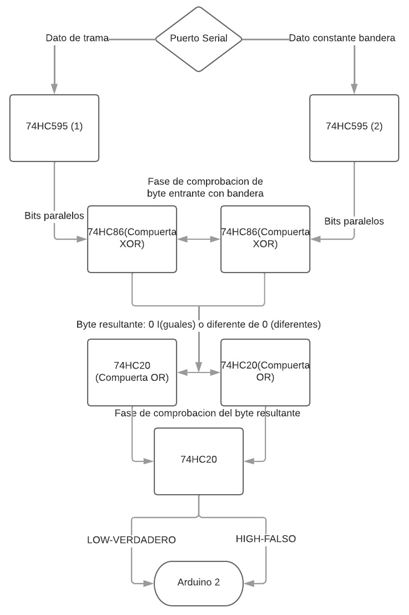
\includegraphics[scale=0.7]{Captura6.JPG}\\


\newpage
\section{MARCO TEÓRICO}
\label{marco}
[20] Investigar y explicar con sus propias palabras cómo utilizar el circuito integrado 74HC595. En esta parte mostrar un ejemplo de uso del circuito integrado primero de forma independiente con pulsadores o switches y luego usando Arduino,y detallar en el informe la utilidad que puede darle a este elemento para la solución del problema.\\

-Es un registro de desplazamiento que cuenta con una entrada en serie y salida en paralelo de 8 bits. Este dispositivo solo funciona con dos valores de tensión 1 y 0, 1 sería el valor +Vcc y 0 un valor muy cercano a 0v.\\

-Se puede tomar como un conversor de serie-paralelo. Como es de suponer la entrada se dará un valor uno detrás de otro, mientras que su salida mostrará todos los entregará a la vez.\\

-Otro factor importante de este componente es que cada vez que se le entreguen datos nuevos el no los va a sobrescribir lo que hará es desplazarlos n posiciones a la derecha, siendo n el número de datos nuevos.\\

-Una de las utilidades que nos puede entregar este elemento para la solución del problema es el clock de latch lo que quiere decir que hasta que no llegue un flanco de subida por el clock de latch los shift registrer no pasan a la salida permitiendo esto organizar los datos con completa libertad sin ir a afectar el circuito.\\

-Para el caso es muy útil ya que si no existiera el latch veríamos todo el proceso de encriptación mientras se organiza, viendo así datos o valores que no son lo que realmente queremos, mientras que con esto podemos ordenar los datos y cuando realmente deseemos mostrarlo.\\

-Otra gran ventaja que es muy útil de este componente es reducir el número de pines que se necesitaría para llevar a cabo una tarea, lo reduce a 3 pines. Si por ejemplo tenemos varios componentes iguales y conectamos la salida del shift a con la señal de siguiente “conectarlos en cascada” podemos incrementar el número de elementos a controlar sin que suba el nuero de pines.\\
\\
\\
\\
\\
\\
\\
\\
\\
\\
\item 1. Ejemplo para el componente con pulsadores y sin Arduino\\

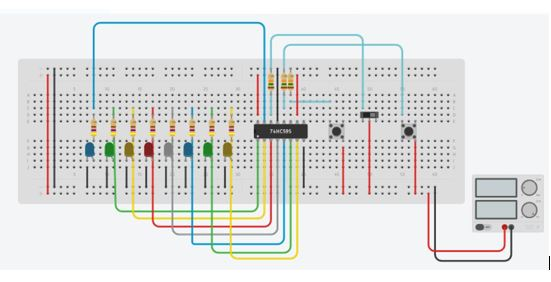
\includegraphics[scale=0.7]{Captura1.JPG}\\
Este es el montaje para ensayar el dispositivo mediante pulsadores y sin uso de arduino.\\

-Le ingresaremos al sistema el siguiente patron para comprobar que si se desplaza a la derecha.\\
PATRON 1011 y tenemos el siguiente resultado.\\
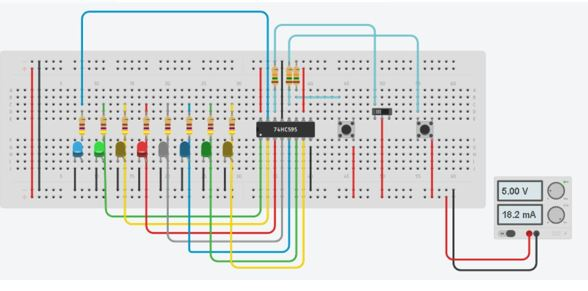
\includegraphics[scale=0.7]{Captura2.JPG}\\
\\
y por ultimo ingresaremos el 0011 para obtener este resultado final.\\
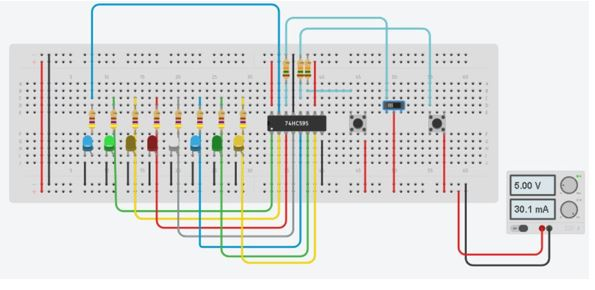
\includegraphics[scale=0.7]{Captura3.JPG}\\
\\
Observando la figura final se puede notar que cada vez que ingresábamos un valor se iba desplazando hacia la derecha, notando así el funcionamiento del componente con ayuda de los pulsadores le indicábamos cual valor mostrar en la salida y cual no.\\
\\
\item 2. Ejemplo usando arduino\\
Montaje\\
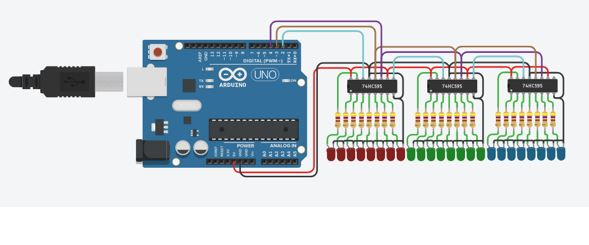
\includegraphics[scale=0.7]{Captura4.JPG}\\
Una vez encendido el arduino se ira encendiendo led por led.\\
\\
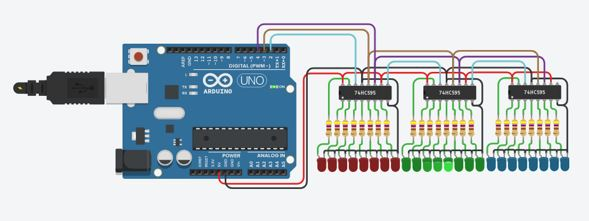
\includegraphics[scale=0.7]{Captura5.JPG}\\
Esto lo hará una y otra vez y como se puede observar en el Arduino se utilizan 3 pines y los componentes están conectados en cascada permitiendo así controlar más cosas al tiempo.\\

Para la comunicación entre los dos arduinos se utilizó los puertos digitales 8 y 9, definiendolos en cada arduino de manera trocada, para que la salida de uno sea la entrada del otro, algo muy importante es que ambos arduinos tengan la tierra común, misma referencia. Añadido a esto se le conecto directamente del circuito a el pin digital 7 del segundo arudino, el lo leerá y si es HIGH es porque va la bandera.\\

También se utilizaron las librerias <SoftwareSerial.h> para el manejo de los puertos de manera serial y en el arduino 2 <LiquidCrystal.h> para el uso de la pantalla LCD.\\

En el arudino 1 se definieron los puertos de la siguiente manera:
const int myserialRX = 8;
const int myserialTX = 9;
SoftwareSerial mySerial(myserialRX, myserialTX);\\

En el arduino 2 así:
const int myserialRX = 9;
const int myserialTX = 8;
SoftwareSerial mySerial(myserialRX, myserialTX);\\

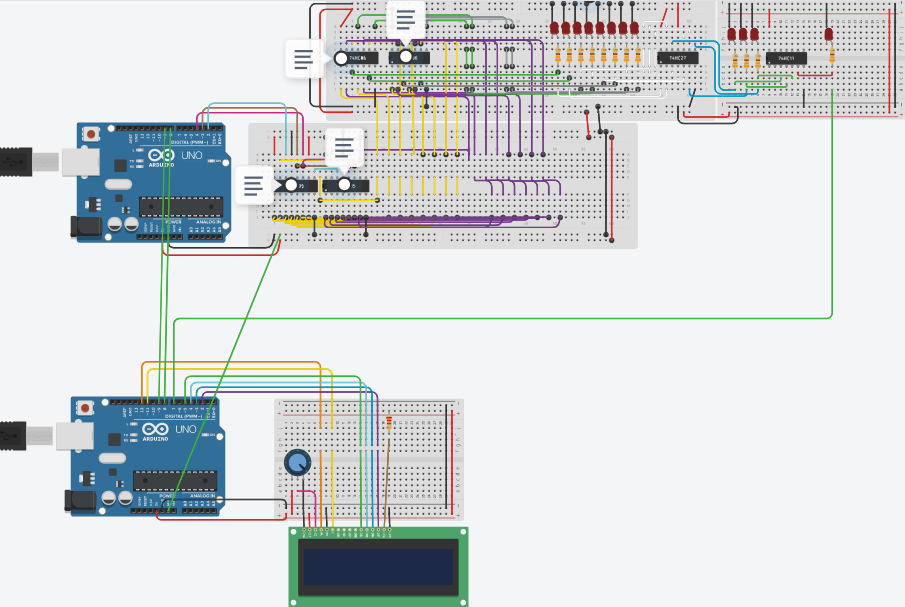
\includegraphics[scale=0.7]{Captura7.PNG}\\

En la imagen anterior, se puede observar la conexión entre los dos arduinos, por medio de los puertos digitales 8 y 9 como se describía anteriormente, También se puede observar que la tierra es común para ambos arduinos.\\

Se puede mirar que el cable que sale del circuito se va directo al puerto digital 7 del otro arduino, el arduino lo recibe y lo lee. comprobando esto que se envian bits.







\newpage
\section{EVOLUCIÓN DEL TRABAJO}
\label{evolucion}
\begin{itemize}
\item El primer inconveniente que se presentó a la hora de resolver el problema fue la comunicación entre los dos arduinos, ya que investigando y buscando como hacer la conexión solo se encontraba información para comunicarlos por puerto serial (RX, TX).Por lo que recurrimos a una asesoría con el monitor del curso el cual nos explicó y en conjunto los comunicamos, luego con ayuda del taller se entendió mejor como era la conexión.

\item Se decidio cambiar de componentes con respecto al diagrama encontrado en análisis del problema, para ahorrarse un componente extra, de esta manera hay menos componentes en el circuito y la simulación será un poco mas fluida.

\item Luego de comparar los datos de entrada con la banera (32), se entregará una señal en alto que irá por un cable conectado directamente al puerto digital (7) del otro Arduino, esto avisandole que ahí va la bandera.

\item Otro de los problemas que surgió , es que se reciben los datos separados por (,) para esto se recurrió a la documentación y se encontró la función (int dato= Serial.parseInt(SKIP ALL)), que lo que hace es entregar el entero asociado y omitir lo demás.

\item A la hora de simular el código en tinkercad, se presentó una curiosidad. Debido a que se tenía que enfocar la parte del circuito encargada de enviar la señal en HIGH cuando aparece el dato bandera, de lo contrario no le avisaba a el otro Arduino que iba el dato bandera; Se perdió tiempo  tratando de solucionar el problema ya que se creía que era un error de conexión o código, pero sin modificar el código ni las conexiones y solo enfocando esa parte funciono correctamente.

\item Una vez recibidos los datos incluyendo el dato bandera (clave) procedemos a desarrollar el código que verificara si se cumplen las reglas de desencriptación.

\item El código final ya está listo y funcional , aunque persiste la inconsistencia en tinkercad debido a que ingresamos un arreglo y no lo hace correctamente, se refresca la página y se introduce nuevamente el mismo arreglo y ahora si el programa funciona. Esto se cree que pasa por la cantidad de componentes usados en el proyecto, porque ya se depuro el código línea por línea y no se encontraron errores.


\end{itemize}

\newpage
\section{CONCLUSIONES}
\label{cONCLUSIONES}
\begin{itemize}
\item Se aprendió a utilizar componentes de los cuales teníamos poco conocimiento, preparandonos esto de mejor manera para seguir enfrentándonos a problemas "reales".
\\

\item El conocimiento sobre el manejo de los diferentes componentes es demasiado importante ya que gracias a ellos se pueden simplificar los problemas y llegar a una solucón más óptima.
\\

\item Fue bastante motivador enfrentarse a un problema que se puede considerar de la vida cotidiana, llevandonos esto a buscar soluciones,leer documentación e infromarnos de la manera correcta todo con el fin de estructurar la solución del problema.
\\

\item Queda por decirlo de alguna manera pendiente realizarlo con el Arduino en mano, debido a que la herramienta de simulación nos presentó varios problemas durante el desarollo de la solución.
\\
\item El trabajar en equipo nos llevó a ser muy organizados con el código, con las conexiones que realizabamos para que el que quisiera avanazar entendiera lo que se realizó previemante. también aprendimos a tener una buena comunicación una buena distribución de tareas aprovechando los fuertes de cada uno pero todo esto sin dejar de estar involucrado en las demás tareas.
\\
\item En algunos momentos se tornó frustrante la situación, sentiamos que no podriamos resolver el problema, pero gracias al trabajo en equipo logramos ir superando los obstaculos y eso fue muy gratificante para nosotros.




\end{itemize}





\end{document}
